\section{Syn3D}
\label{sec:syn3d}
%
%
The academic code, named syn3D, is owned by Professor Siva Nadarajah of McGill University. The program has the following characteristics:
\begin{itemize}
    \item Non-dimensional
    \item Structured
    \item Uses coordinate transformation to generalized curvilinear coordinates
    \item Cell-centered
\end{itemize}
Non-dimensionalization is explained in~\Cref{syn:nondim}, the mesh structure is given in~\Cref{sec:synmesh}, the coordinate transformation method is summarized in~\Cref{sec:transform}, the discretization of the fluid flow and turbulence governing equations are given in~\Cref{sec:synns,sec:synturb} respectively and the wall distance calculation details are given in~\Cref{sec:synwalldist}.
%
\subsection{Non-dimensionalization}
\label{syn:nondim}
%
Round-off errors can be reduced by non-dimensionalizing the governing equations such that all quantities remain in the same order of magnitude. While arbitrary reference quantities can be used, it is convenient to use significant quantities. External flow problems being usually described by free-stream values, the following scaling parameters are used: the airfoil chord length $L$, the free-stream density $\rho_\infty$, the free-stream pressure $p_\infty$, the free-stream dynamic viscosity $\mu_\infty$ and a reference temperature $T_{ref}$. Usage of these scales leads to the following relations between dimensional quantities, now denoted by the superscript $^*$, and non-dimensionalized quantities:
\begin{gather*}
    \rho = \frac{\rho^*}{\rho_\infty}, \quad\quad
    u_i = \frac{u_i^*}{\sqrt{p_\infty/\rho_\infty}}, \quad\quad
    p = \frac{p^*}{p_\infty}, \quad\quad
    i = \frac{i^*}{p_\infty/\rho_\infty}, \\
    x_i = \frac{x_i^*}{L}, \quad\quad
    t = \frac{t^*\sqrt{p_\infty/\rho_\infty}}{L}, \quad\quad
    \Omega = \Omega^*\frac{c}{\sqrt{p_\infty/\rho_\infty}}, \\
    \mu = \frac{\mu^*}{\mu_\infty}, \quad\quad
    \mu_T = \frac{\mu^*_T}{\mu_\infty}, \quad\quad
    \sa = \frac{\sa^*}{\mu_\infty/\rho_\infty}, \quad\quad
    d = \frac{d^*}{L}.
\end{gather*}
It also should be noted that the dynamic viscosity is computed from the temperature using Sutherland's law
\begin{equation*}
    \mu = \frac{C_1 T^{3/2}}{T + S},
\end{equation*}
where $C_1 = 1.461E-6$, $S = 110.3$. The temperature in the previous equation is computed from
\begin{equation*}
    T = T_{ref} \frac{p}{\rho},
\end{equation*}
The free-stream dynamic viscosity is computed in the same manner using $T_{ref}$ in the place of $T$.

Substitution of the non-dimensional relations into~\Cref{eq:fansmass,eq:fansmom,eq:fansenergy}, the Favre-averaged Navier-Stokes equations, and rearranging yields:
\begin{align}
    \Dphi{} &= 0 \\
    \pdiff{\rho\vec{u}}{t}
    + \nabla\cdot(\rho\vec{u}\otimes\vec{u})
    &= -\nabla p + \ndim\nabla\cdot(\tau + \tau^T)
    \\
    \pdiff{\rho E}{t} + \nabla\cdot (\rho \vec{u} H) &=
        \ndim\nabla\cdot \left[
            (\tau + \tau^T) \cdot \vec{u}
        \right]
        - \ndim\nabla\cdot\left(k_{\text{eff}}\nabla T\right) .
\end{align}
The equations are unchanged except for the additional scaling factor $\ndim$ multiplying viscous terms in the momentum and energy equations, where $M_\infty$ is the free-stream Mach number. This also shows that an increase in the Reynolds number will cause a decrease in magnitude of the viscous terms, which is in agreement with the definition of the Reynolds number.

Repeating the process above for the Spalart-Allmaras equation and rearranging the production and destruction terms so as to group terms with common factors results in:
\begin{align}
\begin{split}
    \pdiff{\sa}{t} + \vec{u}\cdot(\nabla\sa) &=
        c_{b1}(1 - f_{t2})\Omega\sa
        + \ndim \left\{
            C_{b1}[(1 - f_{t2})f_{v2} + f_{t2}]\frac{1}{\kappa^2} - c_{w1}f_w
        \right\} \left(\frac{\sa}{d}\right)^2
        \\
        &+ \ndim \frac{1}{\sigma}\nabla\cdot\left[ (\nu + \sa) \nabla\sa \right]
        + \ndim \frac{c_{b2}}{\sigma}\left(\nabla \sa\right)^2.
\end{split}
\label{eq:synsa}
\end{align}
The auxiliary functions require the same treatment:
\begin{gather*}
    r = \text{min} \left[
        \ndim \frac{\sa}{\hat{S}\kappa^2 d^2}, 10
    \right] \\
    \hat{S} = \Omega + \ndim \frac{\sa}{\kappa^2 d^2} f_{v2}.
\end{gather*}
Unmentioned functions as well as constants remain unchanged.
\label{sec:synnondim}
%
\subsection{Computational Grid}
%
\label{sec:synmesh}
Syn3D solves problems on three-dimensional multiblock-structured meshes, making the hexahedron the only acceptable element type. Moreover, a field point is located at the centroid of each element -- it follows that the CVs are all hexahedrons. A general hexahedron CV is shown in~\Cref{fig:hex}. In structured grids, each field point, or CV, is uniquely identified by its $i$, $j$ and $k$ indices. Its neighbors can also be identified by incrementing and decrementing the $i$, $j$ and $k$ indices, which is the main advantage of this method.
%This is illustrated in~\Cref{fig:structured} for the two-dimensional case, where elements are instead quadrilaterals.
A more detailed discussion of grid generation is given in~\cite{blazek2015computational}.
\begin{figure}
\centering
    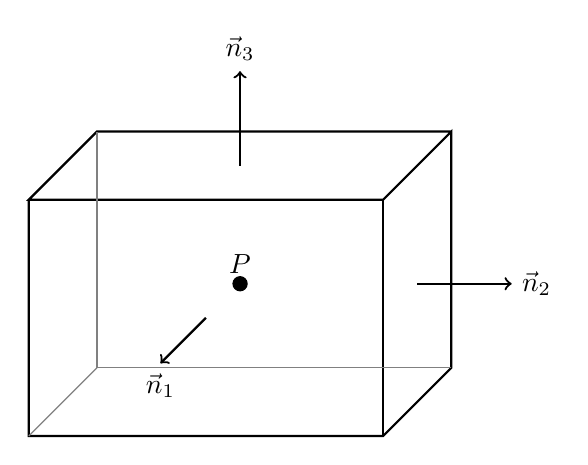
\begin{tikzpicture}[scale=1.5]
  \pgfmathsetmacro{\dx}{3}
  \pgfmathsetmacro{\dy}{2}
  \pgfmathsetmacro{\dz}{1.5}
  \draw[thick](\dx,\dy,0)--(0,\dy,0)--(0,\dy,\dz)--(\dx,\dy,\dz)--(\dx,\dy,0)--(\dx,0,0)--(\dx,0,\dz)--(0,0,\dz)--(0,\dy,\dz);
  \draw[thick](\dx,\dy,\dz)--(\dx,0,\dz);
  \draw[gray](\dx,0,0)--(0,0,0)--(0,\dy,0);
  \draw[gray](0,0,0)--(0,0,\dz);
  \draw[fill] (\dx*0.5, \dy*0.5, \dz*0.5) circle [radius=\dx*0.02] node [above] {$P$};
  \draw[->,thick] (0.5*\dx,0.5*\dy,\dz)
    %node {$\times$} 
    -- (0.5*\dx,0.5*\dy,\dz+1) node [below] {$\vec{n}_1$};
  \draw[->,thick] (\dx,0.5*\dy,0.5*\dz) 
    %node {$\times$} 
    -- (\dx+0.8,0.5*\dy,0.5*\dz) node [right] {$\vec{n}_2$};
  \draw[->,thick] (0.5*\dx,\dy,0.5*\dz) 
    %node {$\times$} 
    -- (0.5*\dx,\dy+0.8,0.5*\dz) node [above] {$\vec{n}_3$};
  %\node at (0.5*\dx, 0.5*\dy, 0.0) {$\times$};
  %\node at (0.0, 0.5*\dy, 0.5*\dz) {$\times$};
  %\node at (0.5*\dx, 0.0, 0.5*\dz) {$\times$};
  % \draw[
  %\node [align=left] at (0.0, -\dy*0.3, \dz) {
    %\begin{tabular}{cl}
   % $\times$ & Integration point\\
    %\tikz\draw[fill] circle (0.5ex); & Field point
    %\end{tabular}  
%};
\end{tikzpicture}
\caption{A hexahedron element. Field point is shown as solid black circle.}\label{fig:hex}
\end{figure}

%\begin{figure}
%\centering
%\begin{tikzpicture}
%  % Use https://www.easycalculation.com/area/polygon-centroid-point.php for centroid
\begin{tikzpicture}[scale=5.0]
  % I lines
  \draw (-0.05,-0.02) -- (0.0,0.0) -- (0.7, 0.03) -- (1.5, 0.0) -- (2.2, 0.0) -- (2.25, -0.02);
  \draw (0.05,0.6) -- (0.1, 0.7) -- (0.68, 0.72) -- (1.53, 0.62) -- (2.15, 0.60) -- (2.2, 0.61);
  \draw (0.0, 1.2) -- (0.05, 1.21) -- (0.83, 1.28) -- (1.58, 1.2) -- (2.2, 1.18) -- (2.25, 1.19);
  \draw (0.03, 1.7) -- (0.08, 1.70) -- (0.77, 1.65) -- (1.5, 1.67) -- (2.12, 1.7) -- (2.17, 1.72);
  % J lines
  \draw (-0.02, -0.05) -- (0.0,0.0) -- (0.1, 0.7) -- (0.05, 1.21) -- (0.08, 1.70) -- (0.06, 1.75);
  \draw (0.79, -0.02) -- (0.7, 0.03) -- (0.68, 0.72) -- (0.83, 1.28) -- (0.77, 1.65) -- (0.79, 1.7);
  \draw (1.49, -0.05) -- (1.5, 0.0) -- (1.53, 0.62) -- (1.58, 1.2) -- (1.5, 1.67) -- (1.52, 1.72);
  \draw (2.19, -0.05) -- (2.2, 0.0) -- (2.15, 0.60) -- (2.2, 1.18) -- (2.12, 1.7) -- (2.11, 1.75);
  % Field points
\draw[fill] (0.370, 0.362) circle [radius=0.02] node [above] {i-1, j-1};
\draw[fill] (0.415, 0.978) circle [radius=0.02] node [above] {i-1, j    };
\draw[fill] (0.432, 1.460) circle [radius=0.02] node [above] {i-1, j+1};
\draw[fill] (1.103, 0.343) circle [radius=0.02] node [above] {i    , j-1};
\draw[fill] (1.155, 0.955) circle [radius=0.02] node [above] {i    , j    };
\draw[fill] (1.170, 1.450) circle [radius=0.02] node [above] {i    , j+1};
\draw[fill] (1.845, 0.305) circle [radius=0.02] node [above] {i+1, j-1};
\draw[fill] (1.865, 0.900) circle [radius=0.02] node [above] {i+1, j    };
\draw[fill] (1.850, 1.438) circle [radius=0.02] node [above] {i+1, j+1};
\end{tikzpicture}
%\end{tikzpicture}
%\caption{Part of a two-dimensional structured grid}
%\label{fig:structured}
%\end{figure}
%
%\subsection{Numerical schemes}
%\label{sec:synnum}
%


%Spatial discretization, temporal discretization and boundary conditions are described in~\Cref{sec:synspace,sec:syntemp,sec:synbc} respectively.
%
\subsection{Coordinate transformation}
\label{sec:transform}
%
%Usage of a structured grid allows Syn3D to use certain numerical schemes that would not be possible to use with unstructured grids. More specifically, it is possible to write the
The governing equations are written in generalized curvilinear coordinates through a transformation from physical space (Cartesian coordinates) to a more convenient computational space (generalized curvilinear coordinates). A curvilinear grid can be represented through a transformation from the Cartesian coordinates $x_i$ ($x$, $y$, $z$ in three dimensions) to curvilinear coordinates $\xi_i$ ($\xi$, $\eta$, $\zeta$ in three dimensions), where each grid line is a line of constant coordinate $\xi_i$. In three dimensions, $\xi$, $\eta$ and $\zeta$ correspond to the index-directions $i$, $j$, $k$ mentioned in~\Cref{sec:synmesh}. \Cref{fig:transformation} illustrates the concept in two dimensions. The transformation is performed by setting the new coordinates to be functions of the Cartesian coordinates, and vice versa:
\begin{equation*}
    \xi_i = \xi_i(x_j), \quad x_i = x_i(\xi_j), \quad j=1,2,3.
\end{equation*}
\begin{figure}
    \centering
    \begin{tikzpicture}
        % http://texample.net/tikz/examples/polar-plot/
% https://tex.stackexchange.com/questions/330580/drawing-a-semicircle-in-tikz
% https://tex.stackexchange.com/questions/66216/draw-arc-in-tikz-when-center-of-circle-is-specified


% Computational
\def\centerarc[#1](#2)(#3:#4:#5)% Syntax: [draw options] (center) (initial angle:final angle:radius)
    { \draw[#1] ($(#2)+({#5*cos(#3)},{#5*sin(#3)})$) arc (#3:#4:#5); }

\foreach \rad in {2,2.5,...,4} {
    \centerarc[](0,0)(90:180:\rad);
}
\foreach \ang in {0,...,7} {
    \draw (\ang*90/7 + 90:2) -- (\ang*90/7 + 90: 4);
}
\node[below] at (180:3) {A};
\node[below right] at (135:2) {B};
\node[right] at (90:3) {C};
\node[above left] at (135:4) {D};

% CSYS
\draw [thick, <->] (0,0.5) node [left] {$y$}
-- (0,0) -- (0.5,0) node [below right] {$x$};


\draw [very thick, ->] (1, 2) -- (2, 2);

\def\xin{3}
\def\xf{6.5}
\def\yin{0.5}
\def\yf{4}
\def\ni{7}
\def\nj{4}
\pgfmathsetmacro{\ys}{(\yf - \yin)/(\nj)}
\pgfmathsetmacro{\xs}{(\xf - \xin)/(\ni)}
\foreach \y in {0,...,\nj} {
    \draw (\xin,\y*\ys + \yin) -- (\xf,\y*\ys + \yin);
}
\foreach \x in {0,...,\ni} {
    \draw (\x*\xs + \xin,\yin) -- (\x*\xs + \xin,\yf);
}
\node[left]  at (\xin,0.5*\yf + 0.5*\yin) {A};
\node[right] at (\xf, 0.5*\yf + 0.5*\yin) {C};
\node[below] at (0.5*\xf + 0.5*\xin,\yin) {B};
\node[above] at (0.5*\xf + 0.5*\xin, \yf) {D};

\draw[very thick] (\xin,\yin-0.1) -- (\xin,\yin-0.4) node [below] {\footnotesize $\text{i}=1$};
\draw[very thick] (\xf,\yin-0.1) -- (\xf,\yin-0.4) node [below] {\footnotesize ~~~~$\text{i}= \text{i}_{\text{max}}$};

\draw[very thick] (\xf+0.1,\yin) -- (\xf+0.4,\yin) node [right] {\footnotesize $\text{j}=1$};
\draw[very thick] (\xf+0.1,\yf) -- (\xf+0.4,\yf) node [right] {\footnotesize $\text{j}= \text{j}_{\text{max}}$};

\draw[thick, <->] (9,0.5) node [left] {$\eta$}
    -- (9,0) -- (9.5,0) node [below right] {$\xi$};
    \end{tikzpicture}
    \caption{Mapping from physical space ($x$, $y$) to computational space ($\xi$, $\eta$)}
    \label{fig:transformation}
\end{figure}

Transformation from physical to computational space is then defined by the metrics:
\begin{equation*}
    K_{nm} = \left[ \pdiff{x_n}{\xi_m} \right], \quad
    J = \text{det}(K), \quad
    K_{nm}^{-1} = \left[ \pdiff{\xi_n}{x_m} \right], \quad n,m = 1, 2, 3.
\end{equation*}

Cartesian derivatives can then be expressed in terms of the curvilinear coordinates using the chain rule:
\begin{equation}
    \pdiff{\phi}{x_j} = K_{ij}^{-1}\pdiff{}{\xi_i},
    \label{eq:transform}
\end{equation}
where implicit summation is used.

A geometrical interpretation of these metric terms can be made. The Jacobian $J$ corresponds to the volume of the cell and the vector $\nabla \xi_k J$ is the directed area of the cell interface normal to the $\xi_k$ direction. The following notation can then be introduced
\begin{gather*}
    \nabla \xi_k J = \vec{S}_k = (S_{k1}, S_{k2}, S_{k3}) \\
    \frac{\vec{S}_k}{|\vec{S}_k|}= \vec{n},
\end{gather*}
where the $\vec{n}$ for the face in the $\xi_k$ direction is chosen and in this case $\vec{n}$ always points towards increasing $\xi_k$.

% \begin{equation}
%     \begin{pmatrix}
%         \pdiff{}{x} \\
%         \pdiff{}{y} \\
%         \pdiff{}{z}
%     \end{pmatrix}
%     =
%     \begin{pmatrix}
%         \pdiff{\xi}{x} & \pdiff{\eta}{x} & \pdiff{\zeta}{x} \\
%         \pdiff{\xi}{y} & \pdiff{\eta}{y} & \pdiff{\zeta}{y} \\
%         \pdiff{\xi}{z} & \pdiff{\eta}{z} & \pdiff{\zeta}{z}
%     \end{pmatrix}
%     \begin{pmatrix}
%         \pdiff{}{\xi} \\
%         \pdiff{}{\eta} \\
%         \pdiff{}{\zeta}
%     \end{pmatrix}
%     \label{eq:transform1}
% \end{equation}
% One can also write the inverse transformation in matrix form:
% \begin{equation}
%     \begin{pmatrix}
%         \pdiff{}{\xi} \\
%         \pdiff{}{\eta} \\
%         \pdiff{}{\zeta}
%     \end{pmatrix}
%     =
%     \begin{pmatrix}
%         \pdiff{x}{\xi} & \pdiff{y}{\xi} & \pdiff{z}{\xi} \\
%         \pdiff{x}{\eta} & \pdiff{y}{\eta} & \pdiff{y}{\eta} \\
%         \pdiff{x}{\zeta} & \pdiff{y}{\zeta} & \pdiff{z}{\zeta}
%     \end{pmatrix}
%     \begin{pmatrix}
%         \pdiff{}{x} \\
%         \pdiff{}{y} \\
%         \pdiff{}{z}
%     \end{pmatrix}
%     \label{eq:transform2}
% \end{equation}
% Elements of the matrix in~\Cref{eq:transform2} can easily be calculated. The metric terms can then be obtained by inverting said matrix for each CV.

Then, given the metric terms, derivatives can be evaluated using simple finite difference methods, which is the primary goal of performing a coordinate transformation. For instance, one can obtain an approximation to $\partial \phi / \partial \xi$ using centered differences:
\begin{equation*}
    \pdiff{\phi}{\xi} = \frac{\phi_{i+1,j,k} - \phi_{i-1,j,k}}{2\Delta \xi},
\end{equation*}
while $\Delta \xi$ is arbitrary, it is typically chosen to be equal to one.

Finally, usage of a curvilinear grid also allows the closed surface integral, where the midpoint method is used as the quadrature, to be written for the CV at coordinate $(i,j,k)$ as:
\begin{align}
    \begin{split}
    \int_{\surf} (\vec{F}\cdot\vec{n})~dS &=
        (\vec{F}\cdot \vec{S}_1)_{i+\frac{1}{2},j,k}
      - (\vec{F}\cdot \vec{S}_1)_{i-\frac{1}{2},j,k} \\
      &+ (\vec{F}\cdot \vec{S}_2)_{i,j+\frac{1}{2},k}
      - (\vec{F}\cdot \vec{S}_2)_{i,j-\frac{1}{2},k} \\
      &+ (\vec{F}\cdot \vec{S}_3)_{i,j,k+\frac{1}{2}}
      - (\vec{F}\cdot \vec{S}_3)_{i,j,k-\frac{1}{2}}.
    \end{split}
    \label{eq:synflux}
\end{align}
The integration points are at the midpoint of each face enclosing the hexahedron CV, which are represented by the $\pm \frac{1}{2}$ increments to indices. The three lines in~\Cref{eq:synflux} on the right-hand side can be seen as the fluxes in the $\xi$, $\eta$ and $\zeta$ directions respectively.
%
\subsection{Discretization of the fluid flow equations}
\label{sec:synns}
%
This section describes the numerical discretization of the Favre-averaged Navier-Stokes equations, namely: temporal discretization, discretization of convective fluxes, discretization of viscous fluxes, artificial dissipation, boundary conditions and convergence acceleration.
%
\subsubsection{Temporal discretization}
%
Syn3D uses the modified Runge-Kutta approach introduced by Jameson \textit{et al.}~\cite{jameson1981numerical} to march the solution in pseudo-time. Let $\vec{W}$ be the vector of conserved variables defined as:
\begin{equation}
    \vec{W} =
    \begin{Bmatrix}
        \rho \\
        \rho u_1 \\
        \rho u_2 \\
        \rho u_3 \\
        \rho E
    \end{Bmatrix}
    \label{eq:wstate},
\end{equation}
and $\vec{R}$ be the residual vector, the modified Runge-Kutta scheme advances the solution at the current time level $\vec{W}^{(n)}$ to the solution at the next time level $\vec{W}^{(n+1)}$ in the following manner:
\begin{align*}
    \vec{W}^{(0)} &= \vec{W}^{(n)} \\
    \vec{W}^{(k)} &= \vec{W}^{(0)} - \alpha_k \Delta t \vec{R}(\vec{W}^{(k-1)}),
        \quad k=1,...,m \\
    \vec{W}^{(n+1)} &= \vec{W}^{(m)},
\end{align*}
where $m$ is the total number of stages and $\vec{R}(\vec{W}^{(k-1)})$ is the residual evaluated using the solution from the previous stage $\vec{W}^{(k-1)}$. Compared to the classical Runge-Kutta methods where the solution at each stage is kept to obtain the solution at the next time level, the modified Runge-Kutta only requires storage of the latest residual and the zeroth solution, which reduces memory requirements.

The dissipative fluxes, which includes viscous fluxes and artificial dissipation, and convective fluxes are treated separately when computing the residual. The residual at each stage can be defined as:
\begin{align*}
    \vec{R}^{(k)} &= \vec{R}_{c}^{(k}) + \vec{R}_{d}^{(k)} \\
    \vec{R}_c^{(k)} &= \vec{R}_c(\vec{W}^{(k)}) \\
    \vec{R}_d^{(k)} &= \beta_k \vec{R}_d(W^{(k)}) + (1 - \beta_k)\vec{R}_d^{(k-1)},
\end{align*}
where $\vec{R}_c$ and $\vec{R}_d$ are the convective and dissipative contributions to the residual respectively. The stage coefficients $\alpha_k$ and blending coefficients $\beta_k$ are chosen such that numerical stability is maximized. In this work, a five stage scheme is employed along with the following coefficients:
\begin{align*}
    \alpha_1 = 0.25 \quad \alpha_2 = 0.1667 \quad \alpha_3 = 0.375
        \quad \alpha_4=0.5 \quad \alpha_5 = 1.0 \\
    \beta_1 = 1,0 \quad \beta_2 = 0.0 \quad \beta_3 = 0,56
        \quad \beta_4 = 0.0 \quad \beta_5 = 0.44.
\end{align*}
%
\subsubsection{Discretization of convective fluxes}
%
Computation of convective fluxes require evaluation of the conserved quantities at cell faces. This is accomplished through simple arithmetic averaging. For instance, let $\vec{F}_c$ be the convected quantity, then its value on the $i+\frac{1}{2}$ face is approximated as:
\begin{equation}
    \vec{F}_{c_{i+\frac{1}{2},j,k}} = \frac{1}{2}\left(
        \vec{F}_{c_{i+1,j,k}} + \vec{F}_{c_{i,j,k}}
    \right)
    \label{eq:synavg}.
\end{equation}
This leads to a three-point stencil in each grid direction. Discretization of the convective fluxes in this manner then results in a seven-point stencil for each CV.
%
\subsubsection{Discretization of pressure}
%
The pressure gradient in the momentum equations is typically written as a source term. However, the term can be treated conservatively by treating it as a surface force and applying the divergence theorem as such:
\begin{equation*}
    \int_\vol \nabla p~d\vol = \int_{\surf} p\vec{n}~dS.
\end{equation*}
The above equation results in a three-dimensional vector with each component belonging to either the $x$-momentum, $y$-momentum and $z$-momentum equations. The integral for the momentum equation in the $m$ Cartesian direction is then discretized according to~\Cref{eq:synflux} with $\vec{F} = p \boldsymbol{i}_m$ and the pressure at integration points is evaluated using~\Cref{eq:synavg}.
%
\subsubsection{Discretization of viscous fluxes}
%
In addition to the evaluation of quantities at each integration point, computation of viscous fluxes also requires computation of derivative terms, which are not available either at the field points or integration points. This is done using two levels of approximation: interpolation and differentiation.

The value of the flux on a given face is approximated by the arithmethic average of the flux quantities at the four vertices sharing this face. For instance, let $\vec{F}_v$ be the viscous flux, then its value on the $i+\frac{1}{2}$ face is approximated as:
\begin{equation*}
    \vec{F}_{v_{i+\half,j,k}} = \frac{1}{4} \left(
        \vec{F}_{v_{i+\half,j+\half,k+\half}} +
        \vec{F}_{v_{i+\half,j-\half,k+\half}} +
        \vec{F}_{v_{i+\half,j+\half,k-\half}} +
        \vec{F}_{v_{i+\half,j-\half,k-\half}}
    \right).
\end{equation*}
\begin{figure}
    \centering
    \begin{tikzpicture}[scale=3.0]
      \foreach \s in {0,1,2} {
    \draw (-0.1,\s) -- (2.1,\s);
    \draw (\s,-0.1) -- (\s,2.1);
}
\def\fieldp[#1](#2)(#3)% Syntax: [loc] (coords) (tex)
    { \draw [fill] (#2) circle [radius=0.02] node [#1] {\scriptsize #3}; }
    
\fieldp[below](0.5,0.5)($i,j$);
\fieldp[above](0.5,1.5)($i,j{+}1$);
\fieldp[below](1.5,0.5)($i{+}1,j$);
\fieldp[above](1.5,1.5)($i{+}1,j{+}1$);

%  \def\intp[#1](#2)(#3) 
%      { \node at (#2) {$\times$}; 
%         \node [#1] at (#2) {#3}; }

% \intp[below](1.0, 0.5)(asd);

\node at (1.0, 0.5) {$\times$};
\node [above right] at (1.0, 0.5) {\scriptsize $i{+}\half,j$};

\draw (1.0, 1.0) node[fill,diamond,scale=0.5]{};
\node [above left] at (1.0, 1.0) {\scriptsize  $i{+}\half,j{+}\half$};

\draw[dashed] (0.5,0.5) -- (0.5, 1.5) -- (1.5, 1.5) -- (1.5, 0.5) -- cycle;

\draw[thick, <->] (-0.8,0.3) node [left] {$\eta$}
    -- (-0.8,0) -- (-0.5,0) node [below right] {$\xi$};
    \end{tikzpicture}
    \caption{Auxiliary control volume (dashed) for the viscous fluxes in two dimensions.}
    \label{fig:synaux}
\end{figure}

An auxiliary control volume is formed at each vertex by joining the centroids of all eight elements that share that vertex. This is illustrated in~\Cref{fig:synaux} for the two-dimensional case. For the sake of conciseness, let the viscous flux $\vec{F}_v$ be of the form $\Gamma \nabla \phi$ -- even though the viscous term in the momentum and energy equations contain more derivatives, they are all calculated in the same manner. The diffusion coefficient value $\Gamma$ at a vertex is approximated by an arithmethic average of the values at field points, which form the vertices of the auxiliary control volume. This can mathematically be written for the vertex at $i+\half,j+\half,k+\half$:
\begin{align*}
    \Gamma_{i+\half,j+\half,k+\half} = \frac{1}{8} (
        \Gamma_{i,j,k} + \Gamma_{i+1,j,k} + \Gamma_{i,j+1,k} + \Gamma_{i+1,j+1,k}&
        \\
        + \Gamma_{i,j,k+1} + \Gamma_{i+1,j,k+1} + \Gamma_{i,j+1,k+1} + \Gamma_{i+1,j+1,k+1}&).
\end{align*}

Gradients $\nabla \phi$ at the vertices are calculated through a transformation to curvilinear coordinates. For example, the $k$-component of the gradient at the vertex mentioned above is written as:
\begin{equation}
    \left[ \pdiff{\phi}{x_k} \right]_{i+\half,j+\half,k+\half} =
        \frac{1}{J_{i+\half,j+\half,k+\half}}
        \left[
            \pdiff{\hat{\phi}_{1n}}{\xi} + \pdiff{\hat{\phi}_{2n}}{\eta} + \pdiff{\hat{\phi}_{3n}}{\zeta}
        \right]_{i+\half,j+\half,k+\half}
    \label{eq:velgradvertex},
\end{equation}
where $J$ is the volume of the auxiliary control volume and is approximated in the same way as $\Gamma$. The gradient components in the computational domain are calculated by taking an average of the centered differences in each direction, which can be written as:
\begin{gather*}
    \left[
        \pdiff{\hat{\phi}_{1n}}{\xi}
    \right]_{i+\half,j+\half,k+\half}
    = \frac{
        (\hat{\phi}_{1n,i+1,j,k} - \hat{\phi}_{1n,i,j,k})
      + (\hat{\phi}_{1n,i+1,j+1,k+1} - \hat{\phi}_{1n,i,j+1,k+1})
    }{4}\\
    + \frac{
        (\hat{\phi}_{1n,i+1,j+1,k} - \hat{\phi}_{1n,i,+1j,k})
      + (\hat{\phi}_{1n,i+1,j,k+1} - \hat{\phi}_{1n,i,j,k+1})
    }{4},
\end{gather*}
where $\hat{\phi}$ is the quantity multiplied with the area-directed normal as such:
\begin{equation*}
    \hat{\phi}_{1n,i,j,k} = S_{1n,i,j,k}\phi_{i,j,k},
\end{equation*}
and the directed area at the field point is obtained by an arithmetic average:
\begin{equation*}
    S_{1n,i,j,k} = \frac{S_{1n,i+\half,j,k} + S_{1n,i-\half,j,k}}{2}.
\end{equation*}
This formulation produces a second-order accurate scheme and the stencil extends over twenty-seven cells since it depends on all field points that share at least one vertex with the CV.
%
\subsubsection{Artificial dissipation and convergence acceleration}
Usage of second-order centered difference schemes is known to admit chequer-board solutions, which leads to odd-even point decoupling. This effect can be prevented by adding artificial dissipation to the equations, which was first shown in~\cite{vonneumann1950method}. This new term does not show itself in the governing equations. Syn3D uses an artificial dissipation scheme first introduced by Jameson, Schmidt and Turkel in~\cite{jameson1981numerical}, and referred to as the JST scheme. Its implementation is described in detail~\cite{nadarajah2003discrete}.

Convergence is accelerated through means of multigrid, residual averaging and local time stepping. Implementation of these are also detailed in~\cite{nadarajah2003discrete}.
%
\subsubsection{Boundary conditions}
%
To facilitate implementation of boundary conditions, syn3D uses the concept of ghost cells, or halo cells, which are additional CVs introduced beyond the physical boundaries. This allows the programmer to treat all interior CVs in exactly the same way when calculating fluxes, irrespective of whether the CV has a face on a boundary. This concept is further explained in~\cite{blazek2015computational}. Field points belonging to interior CVs with a face marked as a physical boundary will be sub-scripted with a $2$ and field points belonging to ghost CVs will be sub-scripted with a $1$. Furthermore, field points one past cell 2 and one past cell 1 will be denoted by a 3 and 0, respectively -- this entails that a second set of ghost cells is introduced.

This work uses three different types of boundary conditions:
\begin{enumerate}
    \item Solid wall
    \item Symmetry plane
    \item Far-field
\end{enumerate}

Physically, solid walls require that flow neither enter or leave the domain, which is also referred to as a no-slip boundary condition. This can be expressed mathematically as:
\begin{equation*}
    \vec{u}|_{wall} = \vec{0}.
\end{equation*}
This can be achieved without any changes to the fluxes mentioned previously by setting the following values for the first level halos:
\begin{gather*}
    \rho_1 = \rho_2 \quad \vec{u}_1 = -\vec{u}_2 \quad p_1 = p_2,
\end{gather*}
and by updating density, velocity, pressure and energy at second level halos according to:
\begin{equation*}
    \phi_0 = \phi_1 + \left(\phi_1 - \phi_2\right),
\end{equation*}
which is simply a linear extrapolation.

Symmetry planes are required if the flow is to be symmetrical with respect to a plane, which requires the following to be true at the interface
\begin{align*}
    \vec{n}\cdot\nabla\phi &= 0 \\
    \vec{n}\cdot\nabla(\vec{u}\cdot\vec{t}) &= 0\\
    \vec{t}\cdot\nabla(\vec{u}\cdot\vec{n}) &= 0,
\end{align*}
where $\vec{t}$ is the vector tangential to the boundary and $\phi$ represents any scalar quantity. This type of boundary condition is easily implemented by setting density, velocity, pressure and energy in the following manner:
\begin{equation*}
    \phi_1 = \phi_2 \quad \phi_0 = \phi_3.
\end{equation*}

Finally, all simulations have to be conducted within a finite bounded domain. However, simulating external flows requires the incoming far-field (free-stream) flow to not be affected by the body under consideration. Far-field boundary conditions are used for this purpose. Because this is not obvious in practice, there are various ways to implement such conditions. The method used in syn3D is described in detail in~\cite{jameson1983solution} and only briefly summarized here. At far-field boundaries, a characteristic based condition using Riemann invariants is imposed. The Riemann invariants can be expressed as:
\begin{align*}
    R_\infty &= \vec{u}_\infty\cdot\vec{n} - \frac{2 c_\infty}{\gamma - 1} \\
    R_e &= \vec{u}_e\cdot\vec{n} + \frac{2 c_\infty}{\gamma - 1},
\end{align*}
where freestream and interior values are denoted by the $\infty$ and $e$ subscripts and $c$ is the speed of sound. The velocity normal to the boundary and the speed of sound can then be expressed as:
\begin{align*}
    \vec{u}\cdot{n} &= \frac{1}{2}(R_\infty + R_e) \\
    c &= \frac{\gamma - 1}{4}(-R_\infty + R_e).
\end{align*}
The velocity at the boundary can then be found using a velocity triangle:
\begin{equation*}
    \vec{u} = \vec{u}_e\cdot\vec{t} + \vec{u}\cdot\vec{n}.
\end{equation*}
Pressure, density and energy are calculated using entropy.
%
%
\subsection{Discretization of turbulent equations}
\label{sec:synturb}
Turbulent models, including the Spalart-Allmaras equation, are discretized differently than the fluid flow equations: are not solved using the finite volume method, but rather the finite difference method. Thus, the differential form, not integration form, of the equation is solved and each derivative is expressed in curvilinear coordinates through application of~\Cref{eq:transform}. It should be noted that field points are still located at the centroids of the hexahedrons. Schemes used for each term in~\Cref{eq:synsa} are detailed in the following sections.

A fully implicit scheme is used to discretize the time derivative and a segregated solve is used to advance the turbulence and fluid flow equations in time, as will also be detailed in the following sections.
%
\subsubsection{Segregated solve}
%
It can be seen that solving the Favre-averaged fluid flow equations requires that another equation be solved, in this case the SA equation. These equations are inherently coupled, since the momentum and energy equations depend on the eddy viscosity obtained from solving the turbulence equation and the turbulence equation itself depends on fluid quantities such as velocity. A common way to approach this problem is to solve each set of equations separately at each time step, which is what is done in syn3D. The procedure is described by the following steps:
\begin{enumerate}
    \item Solve the turbulence equations using the latest solution field.
    \item Update the eddy viscosity and modified eddy viscosity $\sa$.
    \item Solve the fluid flow equations using the same solution field as well as the updated viscosities.
    \item Update the solution field.
\end{enumerate}
This type of procedure is commonly referred to as a segregated solve.
%
\subsubsection{Discretization of production and destruction terms}
The production and destruction terms do not involve derivatives other than the vorticity $\Omega$, which itself requires computation of velocity gradients. The velocity gradients are calculated at the vertices using~\Cref{eq:velgradvertex}. The vorticity magnitude is then evaluated at the vertices and interpolated to the hexahedron centroid through an arithmethic average of all eight vertices of the hexahedron. The remaining computations all rely on readily available quantities stored at the field point of interest.
%
\subsubsection{Discretization of advection term}
The advection term involves the gradient of the modified eddy viscosity, which can be expressed in curvilinear coordinates as:
\begin{align*}
    \vec{u}\cdot(\nabla\sa) &=
        u_x\pdiff{\sa}{x}
        + u_y\pdiff{\sa}{y}
        + u_z\pdiff{\sa}{z} \\
    &=
    u\left[
        \pdiff{\xi}{x}\pdiff{\sa}{\xi} + \pdiff{\eta}{x}\pdiff{\sa}{\eta} +
            \pdiff{\zeta}{x}\pdiff{\sa}{\zeta}
    \right]
    \\
    &+
    v\left[
        \pdiff{\xi}{y}\pdiff{\sa}{\xi} + \pdiff{\eta}{y}\pdiff{\sa}{\eta} +
            \pdiff{\zeta}{y}\pdiff{\sa}{\zeta}
    \right]
    \\
    &+
    w\left[
        \pdiff{\xi}{z}\pdiff{\sa}{\xi} + \pdiff{\eta}{z}\pdiff{\sa}{\eta} +
            \pdiff{\zeta}{z}\pdiff{\sa}{\zeta}
    \right],
\end{align*}
which can be rewritten as
\begin{equation}
    \vec{u}\cdot(\nabla\sa) =  + \pdiff{\sa}{\eta}q_\eta + \pdiff{\sa}{\zeta}q_\zeta
    \label{eq:saadvfd},
\end{equation}
where
\begin{equation*}
    q_{\xi_k} = u\pdiff{\xi_k}{x} + v\pdiff{\xi_k}{y} + w\pdiff{\xi_k}{z}.
\end{equation*}

Each term in the summation, which can be seen as the convective flux in each curvilinear direction, is discretized using a first-order upwinding scheme. For instance, the first term on the right-hand side of~\Cref{eq:saadvfd} is approximated as:
\begin{equation*}
    \pdiff{\sa}{\xi}q_\xi = q_{\xi_{i,j,k}}^+ (\sa_{i,j,k}- \sa_{i-1,j,k})
        + q_{\xi_{i,j,k}}^- ( \sa_{i+1,j,k} - \sa_{i,j,k}),
\end{equation*}
where
\begin{align*}
    q^+ &= \frac{1}{2}(q + |q|) \\
    q^- &= \frac{1}{2}(q - |q|).
\end{align*}

This scheme leads to a three-point stencil in each curvilinear direction.

%
\subsubsection{Discretization of diffusion term}
%
The diffusion term involves the divergence of the gradient. The gradient is first expressed in curvilinear coordinates similarly to the gradient appearing in the convective term. For the sake of conciseness, let $\delta_x$ represent only discretization for the $x$ derivative, namely:
\begin{equation*}
    \pdiff{\sa}{x} = \delta_x =
    \left[
        \pdiff{\xi}{x}\pdiff{\sa}{\xi} + \pdiff{\eta}{x}\pdiff{\sa}{\eta} +
            \pdiff{\zeta}{x}\pdiff{\sa}{\zeta}
    \right].
\end{equation*}
The divergence operator is then also expressed in curvilinear coordinates. Again, looking only at the derivative in the $x$ direction and letting $\Gamma = (\nu + \sa)$ yields:
\begin{equation*}
    \pdiff{}{x}\left[\Gamma\pdiff{\sa}{x}\right]
    =
    \pdiff{\xi}{x}\pdiff{(\Gamma\delta_x)}{\xi}
    + \pdiff{\eta}{x}\pdiff{(\Gamma\delta_x)}{\eta}
    + \pdiff{\zeta}{x}\pdiff{(\Gamma\delta_x)}{\zeta}.
\end{equation*}
Each term on the right-hand side above involves mixed derivatives of the form:
\begin{equation}
    \pdiff{}{\xi_i}\left[
        \Gamma\pdiff{\xi_j}{x}\pdiff{\sa}{\xi_j}
    \right],
\end{equation}
with unequal indices $i$ and $j$. Such terms vanish for orthogonal grids and their magnitudes relative to terms with equal indices depend on the grid non-orthogonality~\cite{ferziger2012computational}. To reduce computations and to obtain a smaller stencil, these cross terms are simply ignored. Consequently, the expression can be expanded to:
\begin{equation*}
    \pdiff{}{x}\left[\Gamma\pdiff{\sa}{x}\right] = \pdiff{\xi}{x}\pdiff{}{\xi}\left[
        \Gamma\pdiff{\sa}{\xi}\pdiff{\xi}{x}
    \right]
    +
    \pdiff{\eta}{x}\pdiff{}{\eta}\left[
        \Gamma\pdiff{\sa}{\eta}\pdiff{\eta}{x}
    \right]
    +
    \pdiff{\zeta}{x}\pdiff{}{\zeta}\left[
        \Gamma\pdiff{\sa}{\zeta}\pdiff{\zeta}{x}
    \right].
\end{equation*}

A flux-like discretization is then used to approximate the outer derivative with respect to curvilinear coordinates such that:
\begin{align*}
    \pdiff{}{x}\left[\Gamma\pdiff{\sa}{x}\right] &=
    \left(\pdiff{\xi}{x}\right)_{i,j,k}\left[
        \left(
            \Gamma\pdiff{\sa}{\xi}\pdiff{\xi}{x}
        \right)_{i+\half,j,k}
        -
        \left(
            \Gamma\pdiff{\sa}{\xi}\pdiff{\xi}{x}
        \right)_{i-\half,j,k}
    \right]
    \\
    &+
    \left(\pdiff{\eta}{x}\right)_{i,j,k}\left[
        \left(
            \Gamma\pdiff{\sa}{\eta}\pdiff{\eta}{x}
        \right)_{i,j+\half,k}
        -
        \left(
            \Gamma\pdiff{\sa}{\eta}\pdiff{\eta}{x}
        \right)_{i,j-\half,k}
    \right]
    \\
    &+
    \left(\pdiff{\zeta}{x}\right)_{i,j,k}\left[
        \left(
            \Gamma\pdiff{\sa}{\zeta}\pdiff{\zeta}{x}
        \right)_{i,j,k+\half}
        -
        \left(
            \Gamma\pdiff{\sa}{\zeta}\pdiff{\zeta}{x}
        \right)_{i,j,k-\half}
    \right].
\end{align*}
Metrics and the diffusion coefficient at the interfaces are obtained using the usual arithmethic average of the two cells that share the interface and the derivatives are obtained using centered differences. For example, the derivative $\partial \sa/\partial \xi$ at $i + \half$ is written as:
\begin{equation*}
    \left(\pdiff{\sa}{\xi}\right)_{i+\half,j,k} =
    \sa_{i+1,j,k} - \sa_{i,j,k}.
\end{equation*}

Discretization of the diffusion then results in a three-point stencil in each direction.
%
\subsubsection{Discretization of anti-diffusion term}
%
The last term to be discretized is the anti-diffusion, which can be expanded as follows if constant coefficients are ignored:
\begin{equation*}
    \left(\nabla \sa\right)^2 = \left[
        \left(\pdiff{\sa}{x}\right)^2
        +\left(\pdiff{\sa}{y}\right)^2
        +\left(\pdiff{\sa}{z}\right)^2
    \right].
\end{equation*}
Each derivative, which results in three terms when expressed in curvilinear coordinates, must then be squared. Similar to the diffusion term, products involving unequal directions are neglected, resulting in:
\begin{align*}
    \left(\nabla \sa\right)^2 &=
    \left(\pdiff{\sa}{\xi}\right)_{i,j,k}\left[
        \left(\pdiff{\xi}{x}\right)^2
        + \left(\pdiff{\xi}{y}\right)^2
        + \left(\pdiff{\xi}{z}\right)^2
    \right]_{i,j,k}
    \\
    &+
        \left(\pdiff{\sa}{\eta}\right)_{i,j,k}\left[
        \left(\pdiff{\eta}{x}\right)^2
        + \left(\pdiff{\eta}{y}\right)^2
        + \left(\pdiff{\eta}{z}\right)^2
    \right]_{i,j,k}
    \\
    &+
        \left(\pdiff{\sa}{\zeta}\right)_{i,j,k}\left[
        \left(\pdiff{\zeta}{x}\right)^2
        + \left(\pdiff{\zeta}{y}\right)^2
        + \left(\pdiff{\zeta}{z}\right)^2
    \right]_{i,j,k}.
\end{align*}
The metrics are required at the field point itself, thus no interpolation is needed. The derivative with respect to curvilinear directions is, once again, obtained with centered differences. The derivative with respect to $\xi$ can then be written as:
\begin{equation*}
    \left(\pdiff{\sa}{\xi}\right)_{i,j,k} = \frac{\sa_{i+1,j,k} - \sa_{i-1,j,k}}{2}.
\end{equation*}
%
\subsubsection{Temporal discretization}
%
The time derivative is discretized using the backward Euler approach mentioned in~\Cref{sec:fvnum}, which when applied to the S-A model yields the following equation for each field point:
\begin{equation*}
    \left[
        \frac{1}{\Delta t^n} + \pdiff{R^n}{\sa}
    \right] \Delta \sa^n = -R^n.
\end{equation*}
Due to the spatial discretization previously described, the residual at each point $(i,j,k)$ depends on values of $\sa$ at $(i,j,k)$ as well as at the following six neighboring field points: $(i+1,j,k)$, $(i-1,j,k)$, $(i,j+1,k)$, $(i,j-1,k)$, $(i,j,k+1)$ and $(i,j,k-1)$. Consequently, the flux Jacobian, $\partial R^n/\partial \sa$ is a very sparse matrix with at most seven entries on each row, including the diagonal. This system can be solved using the Alternating Direction Implicit (ADI) technique detailed in~\cite{blazek2015computational}, which factorizes the implicit operator into three factors. Each factor contains the linearisation for one particular curvilinear direction in the computational space. The matrix for each factor is a tridiagonal matrix, which can be inverted directly at a low computational cost using tridiagonal matrix algorithm, also known as the Thomas algorithm~\cite{thomas1949elliptic}.
%
\subsubsection{Boundary conditions}
%
Implementation of boundary conditions for the turbulence model also benefits from the ghost cell structure previously described. Solid wall boundary conditions are implemented by setting the first level ghost cell as:
\begin{equation*}
    \sa_1 = -\sa_2,
\end{equation*}
which will result in an arithmethic average of zero at the interface.

Symmetry planes are implemented in exactly the same way as for the fluid flow equations, and far-field boundary conditions are implemented as follows:
\begin{align*}
    \sa_1 &= \sa_\infty \quad\text{ingoing flow}\\
    \sa_1 &= \sa_2 \quad \text{outgoing flow},
\end{align*}
where the flow direction is determined by the sign of $\vec{u}\cdot\vec{n}$ at the boundary.

\subsection{Wall distance calculation}
\label{sec:synwalldist}
Syn3D can calculate wall distances either through the brute force approach or the Poisson approach detailed in~\Cref{sec:walldist}. With the brute force approach, distances between each cell center and the nearest face center is calculated. As mentioned in~\Cref{sec:walldist}, this can be a source of error. However, structured meshes are typically constructed in such a way that grid lines are orthogonal to solid wall boundaries, in which case the error vanishes.

The Poisson equation (\Cref{eq:poissondist}) is solved using the Galerkin method, which belongs to the class of finite element techniques. A detailed discussion on using the Galerkin method for solving PDEs can be found in~\cite{reddy1993introduction} and only an overview is given here.

The first step is to rewrite the Poisson equation in the following weak form:
\begin{equation*}
    \int_\vol \left(
        \nabla w\cdot\nabla\phi - w
    \right)~d\vol
    - \int_{\surf} \left[
        (\vec{n}\cdot\nabla\phi)w
    \right]~dS,
\end{equation*}
where $w$ is a ``trial'' function. Since this particular problem only requires homogeneous Dirichlet conditions to be imposed, the second term vanishes. Linear Lagrange shape functions are used as basis functions for $\phi$ as well as $w$. Integrals are approximated using a two-point Gaussian quadrature. This scheme is second-order accurate and results in a linear equation, which is solved using the conjugate gradient method with an algebraic multigrid preconditioner. The PETSc library was used to assemble and solve the linear system~\cite{petsc}. Finally, $d$ is computed at the cell centers by using the shape functions.
